\documentclass[11pt]{article}
\usepackage[utf8]{inputenc}
\usepackage{amsfonts}
\usepackage{amsmath}
\usepackage{float}
\usepackage{tikz}
\usetikzlibrary{automata, positioning, arrows}
\tikzset{
  ->,
  >=stealth',
  node distance=3cm,
  every state/.style={thick, fill=gray!10},
  initial text=$ $,
}

\setlength{\parindent}{0em}
\setlength{\parskip}{1em}

\usepackage{geometry}
\geometry{
  a4paper,
  total={170mm,257mm},
  left=20mm,
  top=20mm,
}

\title{Problem Sheet 4}
\author{Rowan Saunders}
\begin{document}

\begin{titlepage}
	\maketitle
\end{titlepage}

\section{Pumping Lemma}
A lemma is a small theorem, used in mathematics as stepping stones towards
proving bigger results.

The pumping lemma is a statement about regular languages, and we can use it to
prove that certain languages are not regular, because the the pumping lemma does
not apply to them. This is an argument called proof by contradiction.

\subsection{Proof by Contradiction}
Given a statement $S$:

In a proof by contradiction, we assume $S$ is not true. Then we derive something
that is obviously false - a contradiction.
If $S$ being false leads to a contradiction, then $S$ must be true.

The general pattern is as follows:
\begin{quote}
	if $P$ then $Q$, or in mathematics $P \implies Q$

	The contrapositive is true

	if not $Q$ then not $P$, or $\neg Q \implies \neg P$
\end{quote}


\subsection{Pumping Lemma Definition}
\begin{quote}
	Given any regular language $L$, there exists an integer number $n > 0$ (called
	the pumping length) such that any string $w \in L$ with $|w| \geq n$ can be
	represented as $w = x y z$ where:
	\begin{itemize}
		\item $y \neq \varepsilon$
		\item $|xy| \leq n$
		\item $xy^iz \in L$ for all integer $i \geq 0$
	\end{itemize}
\end{quote}

\subsection{Example 1: Finite Language}
Let $L = \{ab, aba\}$

L is regular, as we can write it with the regular expression $ab \cup aba$

The pumping lemma says we can find a pumping length $n$ which meets the
conditions for strings of length $n$ or higher. As this language is finite, it
must have a longest element. In this case, it is "aba", which is length 3 
($|aba| = 3$)

Let $n = 4$, There are no strings in the language $L$ with length greater than
or equal to 4. This statement is considered true by default. This is called
vacuously true.

So, the condition - "every string of length 4 or higher meets some requirements"
- is vacuously true.

If a statement must apply to every element of a set, but the set is empty, then
the statement is considered true.

For example:
\begin{quote}
	\itshape
	Vacuously True:

	Consider the following rule: "if every window on a plane is closed, then it is
	considered safe to take-off".

	A plane with no windows is considered safe.
\end{quote}

The main section of the pumping lemma states that we must be able to repeat the
middle section of any string any number of times, so this can only apply to
infinite languages.

The pumping lemma as a whole still applies to finite languages and thus all
regular languages, because we can always set the pumping length to be one
greater than the longest string in the set.

\subsection{Example 2: Infinite Language}
Let $L = L((ab \cup aba)^\ast)$. As this language can be represented by a
regular expression, the pumping lemma applies.

Consider an example string, and show that it can be pumped:
\begin{quote}
	Let: $w=abaab$ $x=a$ $y=baa$ $z=b$

	Claim: $xy^iz \in L$ (i.e. the main condition of the lemma is satisfied)

	\begin{align*}
		\text{ e.g when } i=0:\quad &ab \in L,\\
		i=1:\quad &abaab \in L,\\
		i=2:\quad &abaabaab \in L, \\
		i=3:\quad &abaabaabaab \in L,\\
		&\text{and so on... }
	\end{align*}
\end{quote}

This was an example of pumping a single string. The lemma state that it will
work for any string. And we will show that and improve the lemma itself next.

\subsection{Proof of the Pumping Lemma}
We can pump $abaab \in L((ab \cup aba)^\ast)$ with $y=baa$

This Language was represented as an NFA, and from which a DFA was determined, in
week 2. Using this DFA (\emph{Figure \ref{fig:pumplemmaproof}}), if you trace the computation of the string abaab, then
it follows a path of 6 states.

\begin{figure}[H]
	\centering
	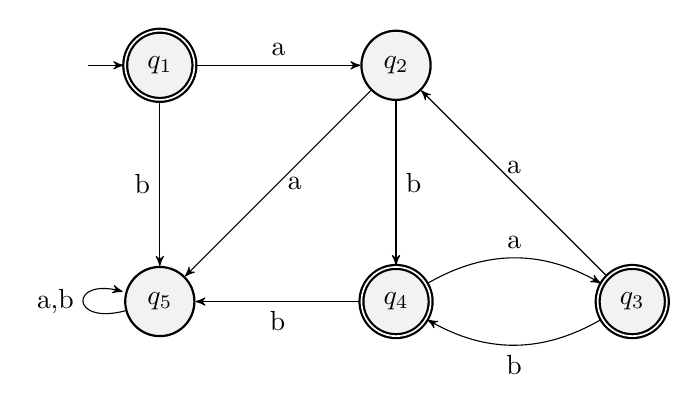
\begin{tikzpicture}
		% states
		\node[state, accepting, initial] (q1) {$q_1$};
		\node[state, right of=q1] (q2) {$q_2$};
		\node[state, accepting, below of=q2] (q4) {$q_4$};
		\node[state, accepting, right of=q4] (q3) {$q_3$};
		\node[state, below of=q1] (q5) {$q_5$};

		% transitions
		\draw (q1) edge[above] node{a} (q2)
		(q1) edge[left] node{b} (q5)
		(q2) edge[right] node{b} (q4)
		(q2) edge[right] node{a} (q5)
		(q3) edge[above] node{a} (q2)
		(q4) edge[bend left,above] node{a} (q3)
		(q3) edge[bend left,below] node{b} (q4)
		(q4) edge[below] node{b} (q5)
		(q5) edge[loop left] node{a,b} (q5);
	\end{tikzpicture}
	\caption{DFA for the language $L((ab \cup aba)^\ast)$}
	\label{fig:pumplemmaproof}
\end{figure}

Notice that for a string of length $x$, the sequence of states the DFA enters is
length $x+1$. There is an initial state, and then x transitions into the next
state of the sequence.

In this DFA, there are only 5 states. The string is of length 5 ($|abaab| = 5$),
So the length of the computation is 6. Therefore, at least one of the five
possible states must be repeated.

The above is an application of something called the pigeonhole principle... If
we put 6 pigeons in 5 holes, then there must be at least one hole with more than
one pigeon.

In this case, there are 2 states that are repeated ($q_2$ and $q_4$). Therefore,
the sequence of strings that leaves $q_2$ and returns to $q_2$ can be be repeated
any number of times, without affecting whether the string is accepted.

We can split the sequence of states (and therefore the input string) into three
sections: The loop between the two occurrences of $q_2$, what came before, and
what came after. This is how the elements x, y and z were chosen from the
previous example.

To finish applying the pumping lemma to this language, we need to set a value
for $n$, the pumping length. Since there are 5 states in this automaton, any
string of length 5 or more will necessarily have a repeated state in its
computation, and so we can repeat the substring that forms as a result.

So for the given language, we can set the pumping length to $n=5$.

We use this idea to prove the pumping lemma itself:
\begin{quote}
	Given any regular language $L$ there must be a DFA $M$ that recognises this
	language.

	Let the pumping length $n$ equal the number of states in $M$

	Consider any string $w \in L$ where $|w| \geq n$.

	The length of the computation of $w$ is: 
	$$|w| + 1$$
	$$|w| \geq n$$
	So
	$$|w| + 1 \geq n + 1$$
	$n$ is equal to the number of states in $M$, so the computation has more steps
	than there are states in $M$

	By the pigeonhole principle, there must be a duplicate state somewhere in the
	first $n+1$ steps of the computation.

	Let's number the states:
	$$q_1, q_2, q_3, ..., q_i, q_j, ..., q_{(n+1)}$$
	Where $q_i = q_j$
	
	Likewise, number the transitions of $w$, where $w_1$ transitions from $q_1$ to
	$q_2$, $w_2$ transitions from $q_2$ to $q_3$ etc.

	The string is then split into three parts
	\begin{itemize}
		\item[] $x$ is the substring from $w_1$ to $w_{(i-1)}$ inclusive. At the
			end of reading $x$, $M$ is in state $q_i$.
		\item[] $y$ is the substring from $w_i$ to $w_{(j-1)}$ inclusive. At the end
			of reading $y$, $M$ is in state $q_j$, which is equal to state $q_i$. Now
			we can repeat $y$ any number of times or skip it, without affecting if the
			string is accepted.
		\item[] $z$ is the remainder of the string from $w_j$ onwards, which must
			take $M$ from state $q_j$ to an accept state, since the original string is
			in the language.
	\end{itemize}

	Notice that while $z$ includes the rest of the string up to the end, $i$ and
	$j$ were both guaranteed to be in the first $n + 1$ states. ($|xy|=j-1$, since
	$j \leq n+1$, $j-1\leq n$). Therefore, the length of $x$ and $y$ combined is
	less than or equal to n ($|xy|\leq n$). This fulfils the final condition of
	the pumping lemma, and hence proving it for any regular language.
\end{quote}

\end{document}
